% --------------------------------------------------------------------
% LaTeX Template for Math Homework
% --------------------------------------------------------------------

\documentclass{article}

% --- PACKAGE IMPORTS ---
% These packages add functionality for math symbols, formatting, etc.
\usepackage[margin=.7in]{geometry}       % For setting page margins
\usepackage{amsmath, amssymb, amsthm}   % American Mathematical Society packages for advanced math
\usepackage{graphicx}                   % For including images
\usepackage{fancyhdr}                   % For creating custom headers and footers
\usepackage[colorlinks=true, urlcolor=blue, linkcolor=blue]{hyperref} % For clickable links
\usepackage{cancel}
\usepackage{array}
\usepackage{amsfonts}
\usepackage{amsxtra}
\usepackage{epsfig}
\usepackage{wasysym}
\usepackage{relsize}
\usepackage{tikz}
\tikzset{every picture/.style={scale=1.2}}
\renewcommand{\normalsize}{\fontsize{12}{20}\selectfont}

% custom commands
\newcommand{\myauthor}{Miguel Gomez}
\newcommand{\canceling}[2]{\textcolor{red}{\cancelto{\textcolor{black}{#1}}{\textcolor{black}{#2}}}}
\newcommand{\todo}[1]{\textcolor{blue}{TODO:#1}}

% --- DOCUMENT & AUTHOR INFORMATION ---
\title{Homework \#2}
\author{
  MATH 3160 -- complex variables\\
  \myauthor
}
\date{Completed: \today}

% --- HEADER & FOOTER CONFIGURATION ---
% This section sets up the header that will appear on each page.
\pagestyle{fancy}
\fancyhf{} % Clears the default header and footer
\lhead{Math 3160 -- HW \#2} % Left side of header
\rhead{\myauthor} % Puts the author's name on the right side
\rfoot{Page \thepage} % Puts the page number on the bottom right

\begin{document}

\maketitle % This command generates the title based on the information above.

% ====================================================================
% --- START OF PROBLEMS ---
% ====================================================================

\section*{Problem 1}
By writing the individual factors on the left in exponential form, performing the needed
operations, and finally changing back to rectangular coordinates, show that

\begin{enumerate}
\item[(a)] $i(1-\sqrt{3}i)(\sqrt{3} + i) = 2(1 + \sqrt{3}i)$
  \begin{align*}
    i &= e^{i\frac{\pi}{2}}\\
    (1-\sqrt{3}i) &= 2\left(\frac{1-\sqrt{3}i}{2}\right) = 2e^{-i\frac{\pi}{3}}\\
    (\sqrt{3} + i)&= 2\left(\frac{\sqrt{3} + i}{2}\right) = 2e^{i\frac{\pi}{6}}\\
    e^{i\frac{\pi}{2}}2e^{i\frac{\pi}{6}}2e^{-i\frac{\pi}{3}} &= 4e^{i\pi\left(\frac{1}{2} + \frac{1}{6} - \frac{1}{3}\right)} \\
      &= 4e^{i\pi\left(\frac{3}{6} + \frac{1}{6} - \frac{2}{6}\right)} \\
      &= 4e^{i\pi\left(\frac{2}{6}\right)}\\ 
      &= 4e^{i\left(\frac{\pi}{3}\right)}\\
      &= 4\left(\frac{1+\sqrt{3}i}{2}\right)\\
    &= 2(1+\sqrt{3}i)\quad \square
  \end{align*}
\hrule
\item[(b)] $\frac{5i}{2+i} = 1+2i$
  \begin{align*}
    \frac{5i}{2+i} &= \frac{5i(2-i)}{(2+i)(2-i)} = \frac{(10i-5i^2)}{4 -2i + 2i -i^2} \\
    &= \frac{(10i-5\canceling{-1}{i^2})}{4 \canceling{0}{-2i + 2i} -\canceling{-1}{i^2}} \quad = \frac{(10i+5)}{5} \\
    &= 1 + 2i \quad \square
  \end{align*}
\hrule
\item[(c)] $(-1 + i)^7 = -8(1+i)$
  \begin{align*}
    -1 + i &= \sqrt{2}\left(\frac{-\sqrt{2}+\sqrt{2}i}{2}\right) = \sqrt{2}e^{i\frac{3\pi}{4}}\\
    (-1 + i)^7 &= (\sqrt{2}e^{i\frac{3\pi}{4}})^7 = \sqrt{2}^7e^{i\frac{21\pi}{4}}\\
           &= \sqrt{2}^7e^{i\frac{21\pi}{4}} = \sqrt{2}^7e^{i\left(\frac{24\pi}{4} - \frac{3\pi}{4}\right)} = \sqrt{2}^7e^{i\left(6\pi - \frac{3\pi}{4}\right)} \\
           &= \sqrt{2}^7\canceling{1}{e^{i6\pi}}e^{-i\left(\frac{3\pi}{4}\right)} = \sqrt{2}^7e^{-i\left(\frac{3\pi}{4}\right)} \\
           &= \sqrt{2}^7\frac{1}{\sqrt{2}}(-1-i) = -2^3(1+i) \\
           &= -8(1+i)\quad \square \\
  \end{align*}
\hrule
\item[(d)] $(1 + \sqrt{3}i)^{-10}= 2^{-11}(-1 + \sqrt{3}i)$
  \begin{align*}
    % Your work here
  \end{align*}
\hrule
\end{enumerate}

\vspace{.5cm} % Space between problems


\newpage
\section*{Problem 2}
Find the square roots of (a) $2i$ and (b) $(1-\sqrt{3}i)$ express them in rectangular coordinates
\newpage
\section*{Problem 3}
Find all roots and indicate in rectangular coordinates
\begin{enumerate}
\item[(a)] $(-16)^{\frac{1}{4}}$
  \begin{align*}
    % Your work here
  \end{align*}
\hrule
\item[(b)] $(-8-8\sqrt{3}i)^{\frac{1}{4}}$
  \begin{align*}
    % Your work here
  \end{align*}
\hrule
\end{enumerate}


\newpage

\section*{Problem 4}
Find the four zeros of $z^4+4$

Converting $z$ into exponential form for $|z| = 1$
 \begin{align*}
 z^4 &= (e^{i\theta})^4 = e^{i4\theta}
 \end{align*}
 Four windings for this, so we should have 4 equally spaced roots that give us the zeros.
 \begin{align*}
   z^4+4 &= 0\\
   z^4 &= -4\\
   \sqrt[4]{z^4} &= \sqrt[4]{-4}\\
   z^{\frac{1}{4}4} &= \sqrt[4]{-4} = e^{\frac{1}{4}i4\theta}\\
   z &= \sqrt[4]{-4} = e^{i\theta}\\
         &= \sqrt[4]{-2\cdot 2} = \sqrt[4]{-\sqrt{2}^2\cdot \sqrt{2}^2} = \sqrt[4]{-\sqrt{2}^4}\\
         &= \sqrt{2}\cdot \sqrt[4]{-1} 
 \end{align*}
 \begin{align*}
   \sqrt{z^4} &= \pm z^2 = \sqrt{-4} = \pm 2\sqrt{-1}\\
   \sqrt{\pm z^2} &= \{\sqrt{z^2}, \sqrt{-z^2}\} = \{\pm z, \pm z\sqrt{-1}\}\\
   &= \{\pm z, \pm zi\}
 \end{align*}
 This is also the following:
 \begin{align*}
   z^4 + 4 &= z^4 - (-4) = z^4 - (i^22^2) = (z^2)^2 - (2i)^2\\
           &=(z^2-2i)(z^2+2i)\\
   \text{converting to exponential}\\
   i &= e^{i\frac{\pi}{2}}\\
   \therefore \sqrt{i} &= (e^{i\frac{\pi}{2}})^{\frac{1}{2}} = e^{i\frac{\pi}{4}}\\
   (z^2-2i) &= (z^2-(\sqrt{2}\sqrt{i})^2) = (z-(\sqrt{2}\sqrt{i}))(z+(\sqrt{2}\sqrt{i}))\\
   &= \boxed{(z-(\sqrt{2}\sqrt{i}))(z+(\sqrt{2}\sqrt{i}))}\\
   \text{similarly, for the positive side}\\
   (z^2+2i) &= (z^2-(-2i)) = (z^2-i^2(\sqrt{2}\sqrt{i})^2)\\
           &= \boxed{(z - (\sqrt{2}\sqrt{i})i)(z+(\sqrt{2}\sqrt{i})i)} \\
   i\sqrt{i} &= e^{\frac{i\pi}{2}}e^{i\frac{\pi}{4}} = e^{i\pi(\frac{1+2}{4})} = e^{i\frac{3\pi}{4}}\\
   \therefore z &=\sqrt{2}\{\pm e^{i\frac{\pi}{4}}, \pm e^{i\frac{3\pi}{4}}\} = \sqrt{2}\{(1+i),(-1+i),(-1-i),(1-i)\}
 \end{align*}
%  Note*: I think this implies that the square root is the angle bisection of a rotation.
 
\newpage

\section*{Problem 5}
Show that if $c$ is an $n^{\text{th}}$ root of 1 other than 1 itself, then:
\begin{align*}
  1 + c + c^2 + &... + c^{n-1} = 0
\end{align*}
Hint: multiply above by $(c-1)$

multiplying the above by $(c-1)$ gives the following
\begin{align*}
  (c-1)\cdot(1 + c + c^2 + &... + c^{n-1}) = (c-1)\cdot 0\\
  c + c^2 + c^3 + &... + c^{n-1} + c^n +\ \ \ \text{ expanding }c \\
  -1 -c -c^2 -&... -c^{n-1} \ \ \ \text{expanding }-1\\
  -1 + (c-c) + (c^2-c^2) + (c^3-c^3) +&... + (c^{n-1}-c^{n-1}) + c^n = 0\\
  -1 + \canceling{0}{(c-c)} + \canceling{0}{(c^2-c^2)} + \canceling{0}{(c^3-c^3)} +&... + \canceling{0}{(c^{n-1}-c^{n-1})} + c^n = 0\\
  -1 + c^n &= 0\\
  c^n &= 1\\
  \sqrt[n]{c^n} &= \sqrt[n]{1}\\
  c &= 1
\end{align*}
Now using something other than 1, i.e. $c\neq 1$, then the sum cannot be 0.
\begin{align*}
  1 + c + c^2 + &... + c^{n-1} = S\\
  \text{same steps as before}&\\
  c^n -1 &= S(c-1)\\
  \text{since }c^n = 1;\ \ &\text{and }c \neq 1\ \ \text{we can divide}\\
  \frac{c^n -1}{c-1} &= S\\
  \text{since }c \neq 1;\ (c-1)\ \text{is not}\ 0 & \text{ but }c^n = 1\\
  \therefore \frac{\canceling{1}{c^n}-1}{c-1} &= \frac{0}{c-1} = S = 0 \quad \square
\end{align*}

 \vspace{1cm}
 \hrule
\newpage

\section*{Problem 6}
For each of the below, indicate the domain of definition.
\begin{enumerate}
\item[(a)] $f(z) = \frac{1}{z^2+1}$

 We need $z^2 + 1 \neq 0$, which means $z^2 \neq -1$.

Solving $z^2 = -1$:
\begin{align*}
z^2 &= -1 = i^2 \\
z &= \pm i\\
(\pm i)^2 + 1 &= i^2 + 1 = -1 + 1 = 0
\end{align*}

undefined only at $z = i$ and $z = -i$.

For all other complex numbers $z$, we have $z^2 + 1 \neq 0$, so the function is well-defined.

$\therefore$ \text{Domain of Definition:} $\mathbb{C} \setminus \{\pm i\}$
 \vspace{1cm}
 \hrule
\item[(b)] $f(z) = \text{Arg}\left(\frac{1}{z}\right)$

  Here we need $z \neq 0$ Since the division is not defined when $z = 0$.

  So for $z$:
\begin{align*}
  \text{Domain of definition: } \mathbb{C} \setminus \{\textbf{0}\}
\end{align*}
This results in the Arg($z$) being defined in the typical range:
\begin{align*}
  -\pi < \text{Arg}(z) \le \pi
\end{align*}
 \vspace{1cm}
 \hrule
  \item[(c)] $f(z) = \frac{z}{z - \bar{z}}$
\begin{align*}
  \text{Recall } z-\bar z &= 2i\text{Im}(z) \\
  \therefore \frac{z}{z - \bar{z}} &= \frac{z}{2i\text{Im}(z)} = \frac{z(-2i\text{Im}(z))}{-(2i\text{Im}(z))^2}\\
                          &=\frac{-2z\text{Im}(z)i}{-(4i^2\text{Im}(z)^2)}=\frac{-2z\text{Im}(z)i}{(4\text{Im}(z)^2)}\\
  \text{Condition: Im}(z) &\neq 0 \\
  \text{Domain of Definition:} \mathbb{C} &\setminus \{z = a+bi\ |\ b = 0;a\in \mathbb{R}\}
\end{align*}
Note*: I mistakenly did this for minus in the denominator, it should be plus after looking over HW sheet again.

\item[(c)] corrected: $f(z) = \frac{z}{z + \bar{z}}$
\begin{align*}
  \text{Recall } z+\bar z &= 2\text{Re}(z) \\
  \therefore \frac{z}{z + \bar{z}} &= \frac{z}{2\text{Re}(z)} \\
  \text{Condition: Re}(z) &\neq 0 \\
  \text{Domain of Definition:} \mathbb{C} &\setminus \{z = a+bi\ |\ a = 0;b\in \mathbb{R}\}
\end{align*}
 \vspace{1cm}
 \hrule
\item[(d)] $f(z) = \frac{1}{(1-|z|^2)}$
  Since $1-|z|^2$ is in the denominator, our condition here is as follows:
  \begin{align*}
    |z|^2 &\neq 1  ; \quad |z| = \sqrt{a^2 + b^2}\\
    |z|^2 &= a^2 + b^2 \\
    a^2 + b^2 &\neq 1
  \end{align*}
  This corresponds to all points on the unit circle.
  \begin{align*}
    \therefore \text{Domain of Definition: }\mathbb{C} \setminus \{|z| = a^2+b^2 = 1\}
  \end{align*}
\end{enumerate}
\newpage
\section{Problem 7}
Sketch the region onto which the sector $r \le 1;\ 0 \le \theta \le \frac{\pi}{4}$ in the $z$-plane is mapped to
 the $w = f(z)$-plane by the transformations
\begin{enumerate}
\item[(a)] $w = z^2$
  
  \begin{align*}
    z &= e^{i\theta} \\
    z^2 &= (e^{i\theta})^2 = e^{i2\theta}  
  \end{align*}
  Corresponds to two windings of the angle $\theta$, essentially moving by $2\theta$ instead:
\begin{center}
\begin{minipage}{0.45\textwidth}
    \centering
    \begin{tikzpicture}
        \draw[->] (-2,0) -- (3,0) node[right] {$\mathbb{R}$};
        \draw[->] (0,-2) -- (0,3) node[above] {$\mathbb{I}$};
        
        % Draw the sector
        \fill[blue!20] (0,0) -- (1,0) arc (0:45:1) -- cycle;
        \draw[thick, blue] (0,0) -- (1,0);
        \draw[thick, blue] (0,0) -- ({cos(45)},{sin(45)});
        \draw[thick, blue] (1,0) arc (0:45:1);
        
        % Grid and labels
        \draw[dashed] (1,0) arc (0:90:1);
        \node at (1,-0.1) {$1$};
        \node at (-0.1,1) {$i$};
        \node at (0.3,0.15) {$\frac{\pi}{4}$};
    \end{tikzpicture}    
    
    $z$-plane
\end{minipage}
\hfill
\begin{minipage}{0.45\textwidth}
    \centering
    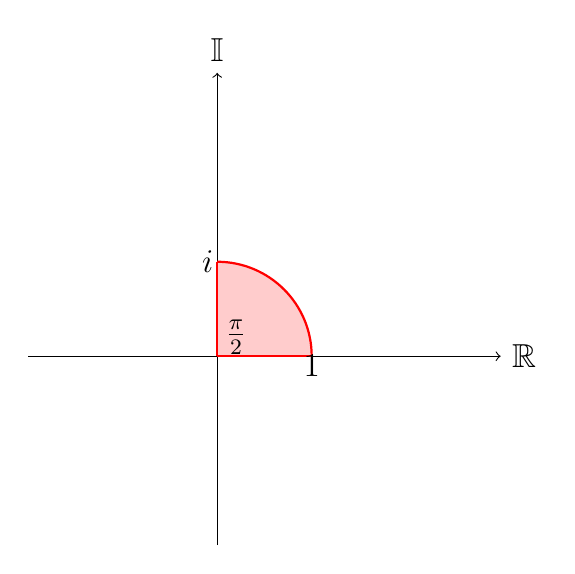
\begin{tikzpicture}
        \draw[->] (-2,0) -- (3,0) node[right] {$\mathbb{R}$};
        \draw[->] (0,-2) -- (0,3) node[above] {$\mathbb{I}$};
        
        % Draw the transformed sector
        \fill[red!20] (0,0) -- (1,0) arc (0:90:1) -- cycle;
        \draw[thick, red] (0,0) -- (1,0);
        \draw[thick, red] (0,0) -- (0,1);
        \draw[thick, red] (1,0) arc (0:90:1);
        
        % Grid and labels  
        \node at (1,-0.1) {$1$};
        \node at (-0.1,1) {$i$};
        \node at (0.2,0.2) {$\frac{\pi}{2}$};
    \end{tikzpicture}
    
    $w$-plane
\end{minipage}
\end{center}\newpage
\item[(b)] $w = z^3$
  Corresponds to three windings of the angle like before but with $3\theta$:
  \begin{center}
\begin{minipage}{0.45\textwidth}
    \centering
    \begin{tikzpicture}
        \draw[->] (-2,0) -- (3,0) node[right] {$\mathbb{R}$};
        \draw[->] (0,-2) -- (0,3) node[above] {$\mathbb{I}$};
        % Add your content for left graph here
        % Draw the sector
        \fill[blue!20] (0,0) -- (1,0) arc (0:45:1) -- cycle;
        \draw[thick, blue] (0,0) -- (1,0);
        \draw[thick, blue] (0,0) -- ({cos(45)},{sin(45)});
        \draw[thick, blue] (1,0) arc (0:45:1);
        
        % Grid and labels
        \draw[dashed] (1,0) arc (0:90:1);
        \node at (1,-0.2) {$1$};
        \node at (-0.2,1) {$i$};
        \node at (0.3,0.15) {$\frac{\pi}{4}$};
    \end{tikzpicture}
    
    \text{$z$-plane}
\end{minipage}
\hfill
\begin{minipage}{0.45\textwidth}
    \centering
    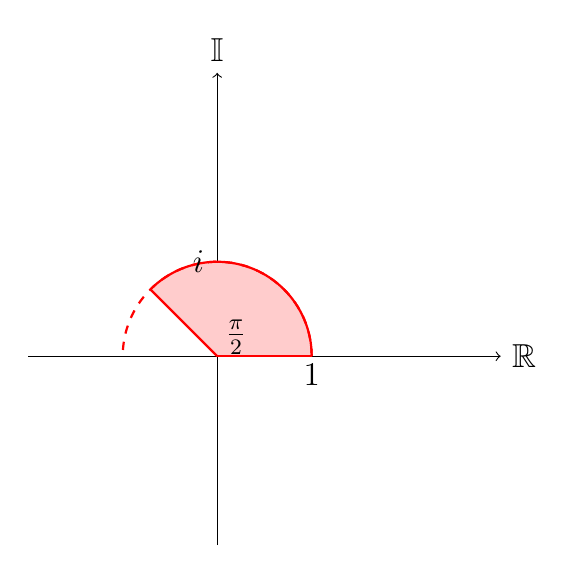
\begin{tikzpicture}
        \draw[->] (-2,0) -- (3,0) node[right] {$\mathbb{R}$};
        \draw[->] (0,-2) -- (0,3) node[above] {$\mathbb{I}$};
        % Add your content for right graph here
        % Draw the transformed sector
        \fill[red!20] (0,0) -- (1,0) arc (0:135:1) -- cycle;
        \fill[red!20] (0,0) -- (1,0) arc (0:135:1) -- cycle;
        \draw[thick, red] (0,0) -- (1,0);
        \draw[thick, red] (0,0) -- (-0.707106781,0.707106781);
        \draw[thick, red] (1,0) arc (0:135:1);
        \draw[dashed, thick, red] (1,0) arc (0:180:1);

        % Grid and labels  
        \node at (1,-0.2) {$1$};
        \node at (-0.2,1) {$i$};
        \node at (0.2,0.2) {$\frac{\pi}{2}$};
    \end{tikzpicture}
    
    \text{$w$-plane}
\end{minipage}
\end{center}
 \vspace{1cm}
 \newpage
\item[(c)] $w = z^4$

  Corresponds to three windings of the angle like before but with $4\theta$:

  \begin{center}
\begin{minipage}{0.45\textwidth}
    \centering
    \begin{tikzpicture}
        \draw[->] (-2,0) -- (3,0) node[right] {$\mathbb{R}$};
        \draw[->] (0,-2) -- (0,3) node[above] {$\mathbb{I}$};
        % Add your content for left graph here
    \end{tikzpicture}
    
    \text{$z$-plane}
\end{minipage}
\hfill
\begin{minipage}{0.45\textwidth}
    \centering
    \begin{tikzpicture}
        \draw[->] (-2,0) -- (3,0) node[right] {$\mathbb{R}$};
        \draw[->] (0,-2) -- (0,3) node[above] {$\mathbb{I}$};
        % Add your content for right graph here
    \end{tikzpicture}
    
    \text{$w$-plane}
\end{minipage}
\end{center}

% \end{enumerate}
% % Add more problems as needed...
% \newpage
% % For graphs/diagrams, you can use TikZ:
% \begin{center}
% \begin{tikzpicture}
%     % Your TikZ code here
%     % Example: Draw axes
%     \draw[->] (-2,0) -- (3,0) node[right] {$\mathbb{R}$};
%     \draw[->] (0,-2) -- (0,3) node[above] {$\mathbb{I}$};
% \end{tikzpicture}
% \end{center}

% %example two planes side by side with minipage
%   \begin{center}
% \begin{minipage}{0.45\textwidth}
%     \centering
%     \begin{tikzpicture}
%         \draw[->] (-2,0) -- (3,0) node[right] {$\mathbb{R}$};
%         \draw[->] (0,-2) -- (0,3) node[above] {$\mathbb{I}$};
%         % Add your content for left graph here
%     \end{tikzpicture}
    
%     \text{$z$-plane}
% \end{minipage}
% \hfill
% \begin{minipage}{0.45\textwidth}
%     \centering
%     \begin{tikzpicture}
%         \draw[->] (-2,0) -- (3,0) node[right] {$\mathbb{R}$};
%         \draw[->] (0,-2) -- (0,3) node[above] {$\mathbb{I}$};
%         % Add your content for right graph here
%     \end{tikzpicture}
    
%     \text{$w$-plane}
% \end{minipage}
% \end{center}


\end{document}

%%% Local Variables:
%%% mode: latex
%%% TeX-master: t
%%% End:
